\documentclass[12pt]{article}
 \usepackage[margin=1in]{geometry}
\usepackage{amsmath,amsthm,mathtools, amssymb,amsfonts,listings,color,graphicx}

\newcommand{\N}{\mathbb{N}}
\newcommand{\Z}{\mathbb{Z}}
\newcommand{\R}{\mathbb{R}}
\newcommand{\E}{\mathbb{E}}
\newcommand{\V}{\mathbb{V}}
\newcommand{\qsum}{\sum\limits_{i=1}^n}

\newcommand{\vpar}{\vspace{.3cm}}

\definecolor{mygreen}{RGB}{28,172,0} % color values Red, Green, Blue
\definecolor{mylilas}{RGB}{170,55,241}

\newenvironment{problem}[2][Problem]{\begin{trivlist}
\item[\hskip \labelsep {\bfseries #1}\hskip \labelsep {\bfseries #2.}]}{\end{trivlist}}
%If you want to title your bold things something different just make another thing exactly like this but replace "problem" with the name of the thing you want, like theorem or lemma or whatever

\begin{document}
\lstset{language=Matlab,%
    %basicstyle=\color{red},
    breaklines=true,%
    morekeywords={matlab2tikz},
    keywordstyle=\color{blue},%
    morekeywords=[2]{1}, keywordstyle=[2]{\color{black}},
    identifierstyle=\color{black},%
    stringstyle=\color{mylilas},
    commentstyle=\color{mygreen},%
    showstringspaces=false,%without this there will be a symbol in the places where there is a space
    numbers=left,%
    numberstyle={\tiny \color{black}},% size of the numbers
    numbersep=9pt, % this defines how far the numbers are from the text
    emph=[1]{for,end,break},emphstyle=[1]\color{red}, %some words to emphasise
    %emph=[2]{word1,word2}, emphstyle=[2]{style},
}





\title{Econ 675: HW 2}
\author{Erin Markiewitz}
\maketitle
\newpage
\tableofcontents
\newpage

\section{Kernel Density Estimation}
\subsection{}


First we consider the kernel density derivative estimator. $\hat{f}(x) =  \frac{1}{nh} \sum\limits_{i=1}^N k \left( \frac{X_i-x}{h} \right)$

The expectation of the estimator is:


\begin{gather*}
  \E[\hat{f}^{(s)}(x)] = \E[\hat{f}^{(s)}(x,h_n)] = \int\limits_{-\infty}^{\infty} \frac{(-1)^{s}}{h^{1+s}} k^{(s)} \left( \frac{z-x}{h} \right) f(z) dz
\end{gather*}


where $k^{(s)}$ is the $s^{th}$ derivative of the kernel function
Now integrate by parts

\begin{gather*}
\int\limits_{-\infty}^{\infty} \frac{(-1)^{s}}{h^{1+s}} k^{(s)} \left( \frac{z-x}{h} \right) f(z) dz =\\
 (-h)k^{(s-1)} \left( \frac{z-x}{h} \right)  f^{(1)}(z) |^\infty_{-\infty} - \int\limits_{-\infty}^{\infty}  \frac{(-1)^{s-1}}{h^{1+s-1}} k^{(s)} \left( \frac{z-x}{h} \right) f^{(1)}(z) dz
\end{gather*}


As $k(.)$ is a $P^{th}$ order kernel function and $s-1<P$, the first term on the RHS of the equation above is equal to zero. Integrating by parts s-1 more times and changing the base, we get the following expression

\begin{gather*}
\int\limits_{-\infty}^{\infty} k \left( u \right) f^{(s)}(uh+x) du
\end{gather*}


So now we take a $P^{th}$ order taylor expansion of $f^{(s)}(uh+x)$ around x, which gives us


\begin{gather*}
f^{(s)}(x) + \frac{1}{P!}\int\limits_{-\infty}^{\infty} k \left( u \right) f^{(s+P)}(uh+x) (uh + x - x)^p du + o(h_n^P)\\
= f^{(s)}(x) + \frac{1}{P!}\int\limits_{-\infty}^{\infty} k \left( u \right) f^{(s+P)}(uh+x) (uh)^p du + o(h_n^P) \\
= f^{(s)}(x) + \frac{f^{(s+P)}(x)}{P!} \mu_P(K) h_n^p +o(h_n^p)
\end{gather*}

where $ \mu_P(K) = \int_\R u^P K(u) du $ - which gives the result. (Note: the second term is the bias of the estimator)

\vpar

Now consider the variance of the estimator

\begin{gather*}
  \V[\hat{f}^{(s)}(x)] = \frac{1}{nh^{2+2s}} \V\left[[k^{(s)} \left( \frac{z-x}{h} \right)\right] = \frac{1}{nh^{2+2s}} \E\left[k^{(s)} \left( \frac{z-x}{h} \right)\right]^2 - \frac{1}{n} \E\left[\frac{1}{nh^{1+s}} k^{(s)} \left( \frac{z-x}{h} \right)\right]^2
\end{gather*}

Now using our derivation of the expected value of our estimator we can rewrite the expression above as:
\begin{gather*}
\frac{1}{nh^{2+2s}} \E\left[k^{(s)} \left( \frac{z-x}{h} \right)\right]^2 - \frac{1}{n}f^{(s)}(x)^2 + O\left(\frac{1}{n}\right)
\end{gather*}

(This comes from $\{ \frac{f^{(s+P)}(x)}{P!} \mu_P(K) h_n^p +o(h_n^p)\}$ being bounded)

So continuing on, we just expand the first term a bit

\begin{gather*}
\V[\hat{f}^{(s)}(x)] = \frac{1}{nh^{2+2s}} \int\limits_{-\infty}^{\infty} k^{(s)} \left( \frac{z-x}{h} \right)^2 f(z) dz - \frac{1}{n}f^{(s)}(x)^2 + O\left(\frac{1}{n}\right) \\
 = \frac{1}{nh^{1+2s}}  \int\limits_{-\infty}^{\infty} k^{(s)} \left( u \right) f(uh+x) du  - \frac{1}{n}f^{(s)}(x)^2 + O\left(\frac{1}{n}\right)  \\
 = \frac{f(x)}{nh^{1+2s}}  \int\limits_{-\infty}^{\infty} k^{(s)} \left( u \right) du  - \frac{1}{n}f^{(s)}(x)^2 + O\left(\frac{1}{n}\right)  \\
  = \frac{f(x) \nu_s(k) }{nh^{1+2s}}- \frac{1}{n}f^{(s)}(x)^2 + O\left(\frac{1}{n}\right)  \\
\end{gather*}

where $\nu_s(k) = \int\limits_\R k^{(s)} \left( u \right)^2 du $ is the roughness of the $s^{th}$ derivative of a given function $k$. Not that the variance is $O(1/n)$ and as $1/n>1/nh_n^{2s+1}$, so that means the statement above is equivalent to

\begin{gather*}
\V[\hat{f}^{(s)}(x)] = \frac{f(x) \nu_s(k) }{nh^{1+2s}}- \frac{1}{n}f^{(s)}(x)^2 + O\left(\frac{1}{n}\right)
\end{gather*}
   which gives the result.






\subsection{}

The optimal bandwith estimator solves the following problem
\begin{gather*}
\text{min}_h \text{   } AIMSE[h] = \text{min}_h \text{   } \int\limits_{-\infty}^{\infty} \left[ \left( h_n^p \mu_p(k) \frac{f^{(P+s)}(x)}{P!} \right)^2 + \frac{\nu_s(k) f(x)}{nh_n^{1+2s}} \right] dx
\end{gather*}

Take first order conditions

\begin{gather*}
0 =  2P h^{2P-1} \int\limits_{-\infty}^{\infty} \left[ \left( \mu_p(k) \frac{f^{(P+s)}(x)}{P!} \right)^2 - \frac{(1+2s) \nu_s(k) f(x)}{nh^{2s}} \right] dx\\
\end{gather*}


\begin{gather*}
\frac{2Pnh^{1-2P-2s}}{(1+2s) \nu_s(k)} = \left( \frac{P!}{\mu_p(k) \nu_{(P+s)}(f))} \right)^2\\
h_{AIMSE,s} = \left( \frac{ (1+2s) \nu_s(k) (P!)^2     }{ 2Pn \mu_p(k)^2 \nu_{(P+s)}(f))} \right)^{\frac{1}{1-2P-2s}}\\
h_{AIMSE,s} = \left( \frac{(1+2s)  (P!)^2     }{2Pn}     \frac{\nu_s(k)}{  \mu_p(k)^2 \nu_{(P+s)}(f))} \right)^{\frac{1}{1-2P-2s}}\\
\end{gather*}


Now for a consistent bandwith estimator we use cross validation procedure from the lecture notes. Cross-Validation minimizes the estimated mean-squared error through a choice of bandwith.

\begin{gather*}
h^* = \text{argmin}_{h \in \R^{++}} \text{   } CV(h) = \frac{1}{n^2h} \sum\limits_{i=1}^n \sum\limits_{j=1}^n K\left( \frac{X_i - X_j}{h}\right) K\left( \frac{X_i - X_j}{h} \right) - \frac{2}{n} \sum\limits_{i=1}^n \hat{f}_{-i}(X_i)
\end{gather*}

where $\hat{f}_{-i}(X_i)$ is the estimated density w/o $x_i$ in the sample.

\subsection{}
\subsubsection{}

We can calculate the optimal bandwith by hand using the equation above for an Epanechnikov kernel, with n = 1000, s = 0 for the following gaussian mixture dgp.


\begin{gather*}
x_i ~ 0.5 N(-1.5,1.5) + 0.5 N(1,1)
\end{gather*}

So the optimal bandwith is

\begin{gather*}
h_{AIMSE,s} = \left( \frac{ 1   }{1000}     \frac{\nu_0s(k)}{  \mu_2(k)^2 \nu_{(2)}(f))} \right)^{\frac{1}{1-4}}\\
\end{gather*}

From the first chapter of Hansen's chapter 1 notes: we now that $\nu(K) = 3/5$ and $\mu_2(K)  = 1/5$. Next as the second derivative of the normal density is

\begin{gather*}
\phi^{(2)}(\mu,\sigma^2) = \frac{1}{2n\sigma^2} e^{- \frac{x-\mu}{\sigma}} \left( \left(\frac{x-\mu}{\sigma}\right)^2 - \frac{1}{\sigma^2}\right)
\end{gather*}


So we can rewrite

\begin{gather*}
  \nu_{(2)}(f)) = \int\limits_{-\infty}^{\infty} \left( 0.5\phi^{(2)}(-1.5,1.5) + 0.5\phi^{(2)}(1,1)  \right)^2 dx
\end{gather*}

Which gives us a $h_{AIMSE,s} = 0.82$


\subsubsection{}

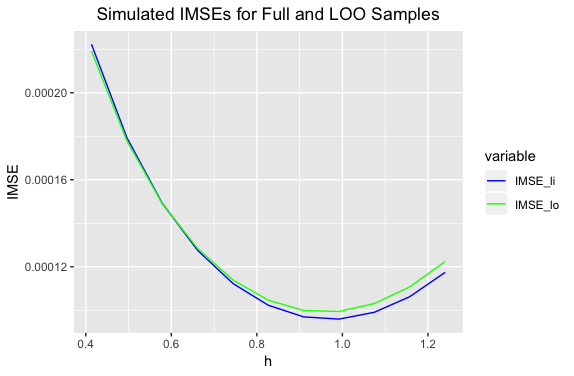
\includegraphics[totalheight=6cm]{rplot_hw2_q1.png}
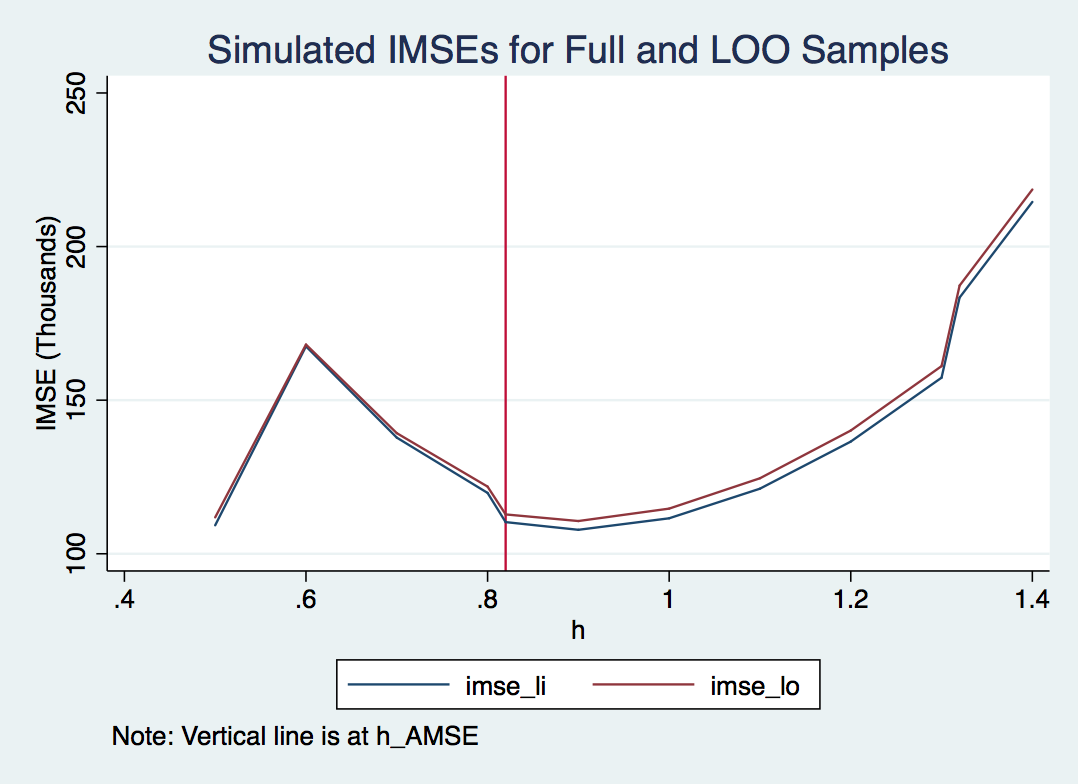
\includegraphics[totalheight=6cm]{hw2q1_3.png}

It appears that the two monte carlo experiments in stata and r do a reasonable job at converging to the theoretically optimal bandwith. Although, they are both slightly off. Although theoretically the two numbers should converge as M $\rightarrow \infty$,


\subsubsection{}
Considering a rule-of-thumbs estimate of the bandwith, we assume the DGP is gaussian, so using the equation from 1.3.1 we find that.

\begin{gather*}
\bar{h}_{AIMSE} = M^{-1} \sum_{m=1}^M  \hat{h}_{AIMSE,m} =
\end{gather*}





\newpage
\section{Linear Smoothing, Cross-Validation and Series}
\subsection{}

Local polynomial regression solves the following problem:

\begin{gather*}
\hat{\beta}_{LPR} =  \text{argmin}_{\beta \in \R^P+1} \text{    } \frac{1}{n}\sum\limits_{i=1}^N \left(Y_i - r_p(x-x)\beta  \right)^2 K(\frac{x_i - x}{h})
\end{gather*}

where $ r_p(u) =(1,u,u^2,...,u^p)' $ The true regression function $e(x_i)$ is estimated by $\hat{e}(x) = \hat{\beta}_{LPR}$, which can be rewritten as a weighted least-squares problem where $ \hat{\beta}_{LPR}(x) = \mathbf{ (R_p' W R_p)^{-1} R_p'WY } $  where the weighting matrix is a diagonal matrix with the kernel functions of the $ x_i $.

where

\begin{gather*}
\mathbf{R}_p = \begin{bmatrix}
1 & (x_1 - x) & (x_1 - x)^2 & \cdots & (x_1 - x)^p \\
\vdots & \cdots & \ddots & \ddots & \vdots \\
1 & (x_n - x) & \cdots & \cdots & (x_n - x)^p \\
\end{bmatrix}
\end{gather*}

and $\mathbf{W}$ is a matrix with kernel weights of $x_i$s on the diagonal

\begin{gather*}
\mathbf{W}  = \begin{bmatrix}
K(\frac{x_1 - x}{h}) & 0 & 0 & 0 \\
0 & K(\frac{x_2 - x}{h}) & 0 & 0 \\
0 & 0 & \ddots & 0 \\
0 & 0 & 0 & K(\frac{x_n - x}{h})  \\
\end{bmatrix}
\end{gather*}

So we can rewrite the estimator of our regression equation as

$\hat{e}(x) = \mathbf{e_1'}\hat{beta_{LPR}} = R_p' W R_p)^{-1} R_p'WY$

where $\mathbf{e_1}$ is a basis vector of length $1+p$.

Therefore we can rewrite the estimator above as a sum.
\begin{gather*}
\hat{e}(x) = \mathbf{e_1'}\left(\sum\limits_{i=1}^n r_p(x_i-x)r_p(x_i-x)'K\left(\frac{x_i - x}{h}\right)\right)^{-1} \left( \sum\limits_{i=1}^n r_p(x_i-x)r_p(x_i-x)y_iK\left(\frac{x_i - x}{h}\right) \right)
\end{gather*}







Now we consider the series estimator, which solves the following problem
\begin{gather*}
\hat{\beta_s} =  \text{argmin}_{\beta \in \R^{k_n}} \text{    } \frac{1}{n}\sum\limits_{i=1}^N \left(Y_i - r_{k_n}(x)\beta  \right)^2 K(\frac{x_i - x}{h})
\end{gather*}

where $r_{k_n}(x)$ is the basis of some series defined on x, so that

\begin{gather*}
\hat{e}(x) = \mathbf{r_{k_n}(x)'\hat{\beta}}
\end{gather*}

where

\begin{gather*}
\mathbf{\hat{beta}_s} = \mathbf{\left( R_p'R_p \right)^{-1}R_pY}
\end{gather*}

and

\begin{gather*}
\mathbf{R}_p = \begin{bmatrix}
1 & x_1 & x_1^2 & \cdots & x_1^p \\
\vdots & \cdots & \ddots & \ddots & \vdots \\
1 & x_n & \cdots & \cdots & x_n^p \\
\end{bmatrix}
\end{gather*}

So we can rewrite the estimated regression function as

\begin{gather*}
\hat{e}(x) = \mathbf{r_p(x)'\left( R_p'R_p \right)^{-1}R_pY}
\end{gather*}

and

\begin{gather*}
\hat{e}(x) = \mathbf{r_p(x)'} \left(\sum\limits_{i=1}^n r_p(x_i)r_p(x_i)'\right)^{-1} \left( \sum\limits_{i=1}^n r_p(x_i)y_i\right)
\end{gather*}


\subsection{}

Next, we need to show the following simplified cross-validation formula holds for local polynomial regression and series estimation:

\begin{gather*}
CV(c) = \frac{1}{n} \sum\limits_{i=1}^n (y_i - \hat{e}(x_i))^2  =  \frac{1}{n} \sum\limits_{i=1}^n \left( \frac{y_i - \hat{e}_{(i)}(x_i)} {1-w_{n,1}(x_i)} \right)^2
\end{gather*}

where c is a tuning parameter ($h_n$ for LPR or a truncation K for series estimators)

Note from the first part of the question, we found that we can right both regressor estimators as a weighted average of the outcome variable

\begin{gather*}
\hat{e}(x) = \frac{1}{n} \qsum w_{n,i}(x)y_i
\end{gather*}
where $w_{n,i}(x) = w_{n,i}(x_1, x_s, \cdots, x_n;x)$

Now in estimation of the tuning parameter, we need our smoothing parameter $w_{n,i}$ to be consistent when we "leave one ($x_i$) out" for estimation. Our smoothing parameter sums to one in the case of the LPR and series estimators. So for cross validation, we need to adjust accordingly.


\begin{gather*}
\hat{e}_{(i)}(x) = \frac{1}{1-w_{ii}} \sum\limits_{i=1}^n w_{i,j}(x)y_i
\end{gather*}

So to get our result:

\begin{align*}
(1-w_{ii}) \hat{e}_{(i)}(x) & = \sum\limits_{j\neq i,j=1}^n w_{i,j}(x)y_j \\
\hat{e}_{(i)}(x) &= \sum\limits_{j\neq i,j=1}^n w_{i,j}(x)y_j + w_{i,i}\hat{e}_{(i)}(x) \\
  &= \sum\limits_{i=1}^n w_{i,j}(x)y_i + w_{ii}\hat{e}_{(i)}(x) - w_{i,i}y_i \\
&= \hat{e}(x) + w_{ii}\hat{e}_{(i)}(x) - w_{i,i}y_i \\
\end{align*}

Which gives us

\begin{align*}
y_i - \hat{e}_{(i)}(x) &= y_i - \hat{e}_(x) - w_{i,i}\hat{e}_{(i)}(x) + w_{i,i}y_i\\
y_i - \hat{e}_{(i)}(x) &= y_i - \hat{e}_(x) w_{i,i}(y_i - \hat{e}_{(i)}(x))\\
(1 - w_{i,i}) ( y_i - \hat{e}_{(i)}(x))  &= y_i - \hat{e}_(x)\\
y_i - \hat{e}_{(i)}(x)  &= \frac{y_i - \hat{e}_(x)}{1-w_{i,i}}\\
\end{align*}

So it follows

\begin{gather*}
\frac{1}{n} \sum\limits_{i=1}^n (y_i - \hat{e}(x_i))^2  =  \frac{1}{n} \sum\limits_{i=1}^n \left( \frac{y_i - \hat{e}_{(i)}(x_i)} {1-w_{n,1}(x_i)} \right)^2
\end{gather*}

\subsection{}

If we assume the data is iid and a finite first moment, we can show consistency:

\begin{align*}
\E[\hat{e}(x) | x] &= \E\left[\qsum w_{n,i}(x_i)y_i\right]\\
&= \qsum w_{n,i}(x_i)\E[y_i | x ]\\
&= \E[y_i | x ]\\
\end{align*}

as $ \qsum w_{n,i}(x_i) = 1 $


Now if we assume a finite second moment of our regressor estimator

\begin{align*}
\V[\hat{e}(x) | x] &= \V \left[\qsum w_{n,i}(x_i)y_i\right]\\
&= \qsum \V[w_{n,i}(x_i)y_i | x ]\\
&= \qsum w_{n,i}(x_i)^2 \V[y_i | x ]\\
&= \V[y_i | x ] \qsum w_{n,i}(x_i)^2 \\
\end{align*}


So the variance estimator is

\begin{align*}
\hat{V}&(x) = \left(\frac{1}{1-n} \qsum (y_i - \hat{e}(x_i))^2 \right) \left( \qsum w_{n,i}(x_i)^2\right)
\end{align*}

Asymptotic normality follows from the CLT

\subsection{}

The

A pointwise asymptotically valid confidence interval for a fixed x is

\begin{gather*}
CI_{95} = \left[\hat{e}(x)  - 1.96  \sqrt{\hat{V}(x) / n}  ; \hat{e}(x)  + 1.96  \sqrt{\hat{V}(x) / n}  \right]
\end{gather*}

but this convidence invterval is not asymptotically valid across the entire support. In order for the confidence interval to be uniformly aymptotically valid we need the interval to hold across the entire support of x

\begin{gather*}
  \text{sup}_{x\in X} \left| \frac{\hat{e}(x) - e(x))}{\sqrt{\hat{V}(x)}} \right| \leq q_{1-\alpha/2}
\end{gather*}



\subsection{}
\subsubsection{}
\subsubsection{}
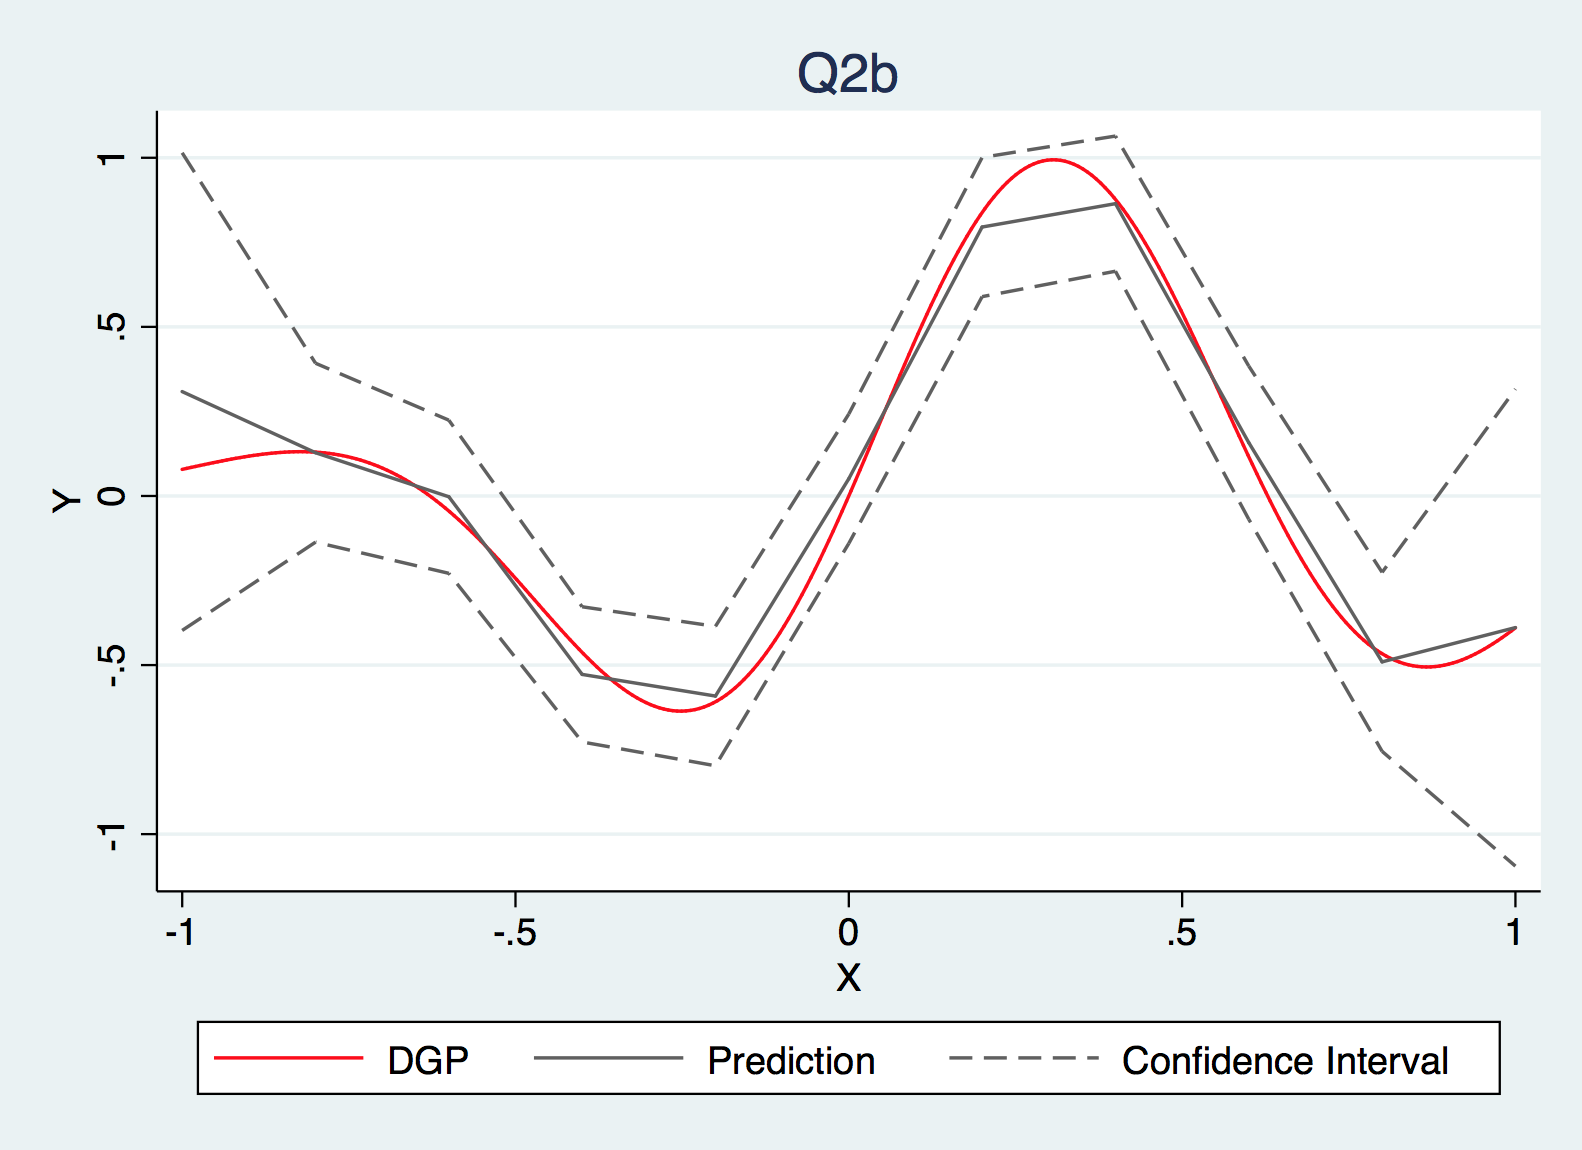
\includegraphics[totalheight=4cm]{pset2q2b.png}
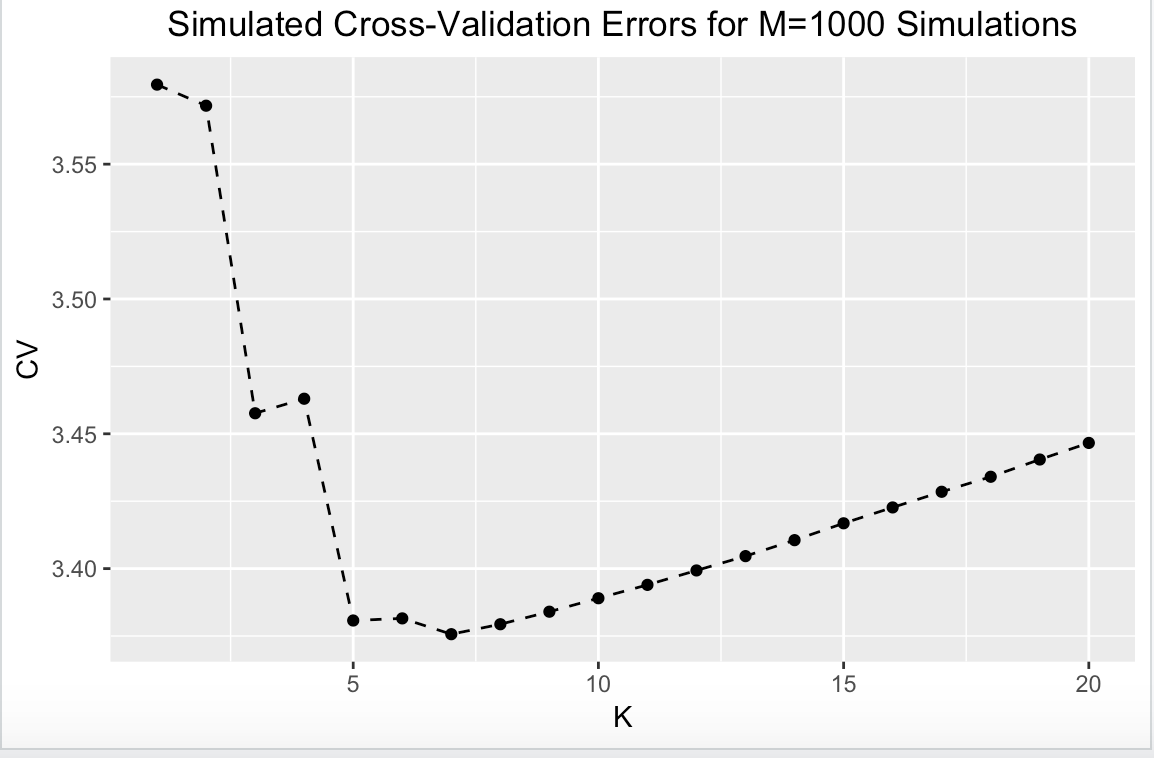
\includegraphics[totalheight=4cm]{pset2q2c_r.png}\\
The two cross validation results from stata and R match up pretty closely.

\subsubsection{}
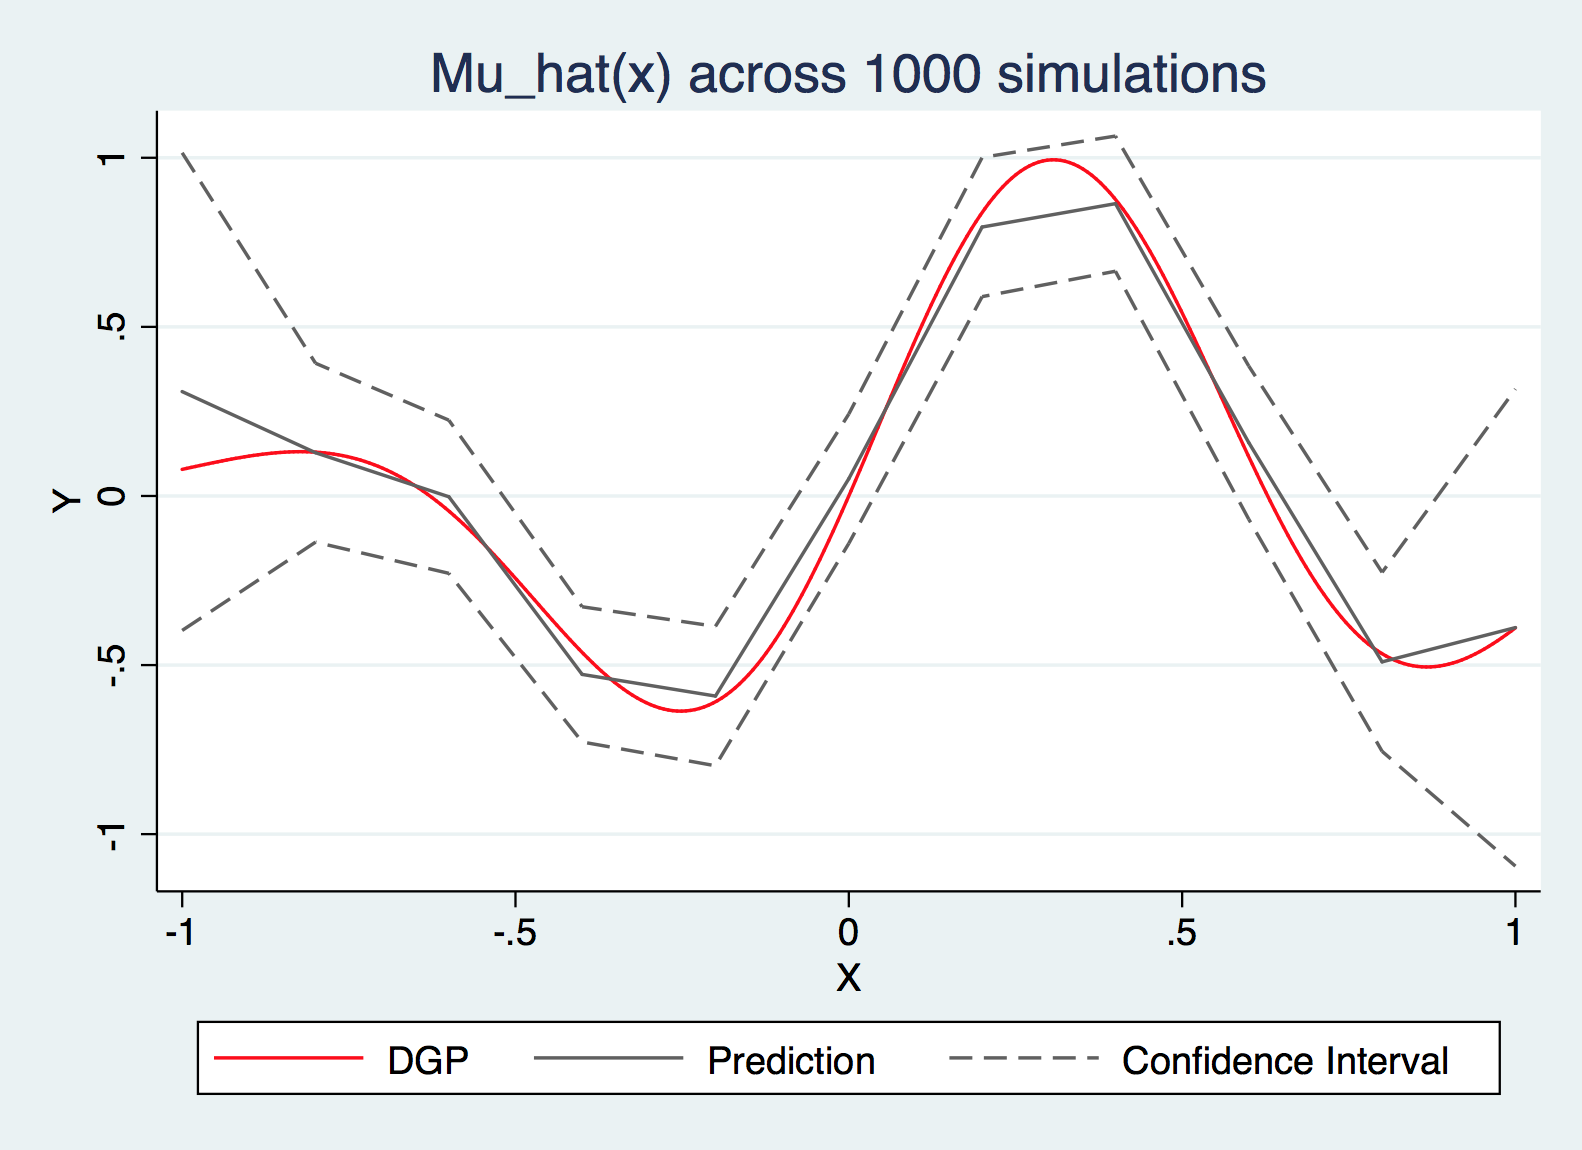
\includegraphics[totalheight=4cm]{pset2q2c.png}
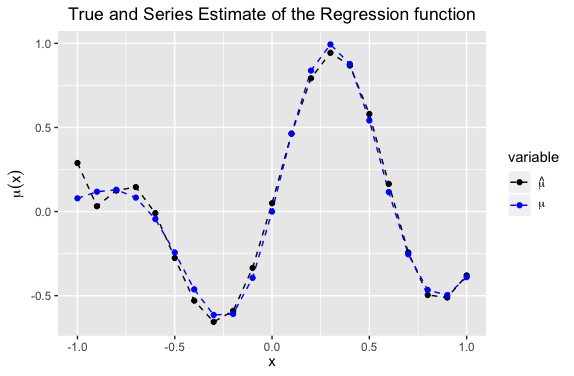
\includegraphics[totalheight=4cm]{pset2q2c11_r.png}\\
The two kernel estimatation results from stata and R match up pretty closely.
\subsubsection{}
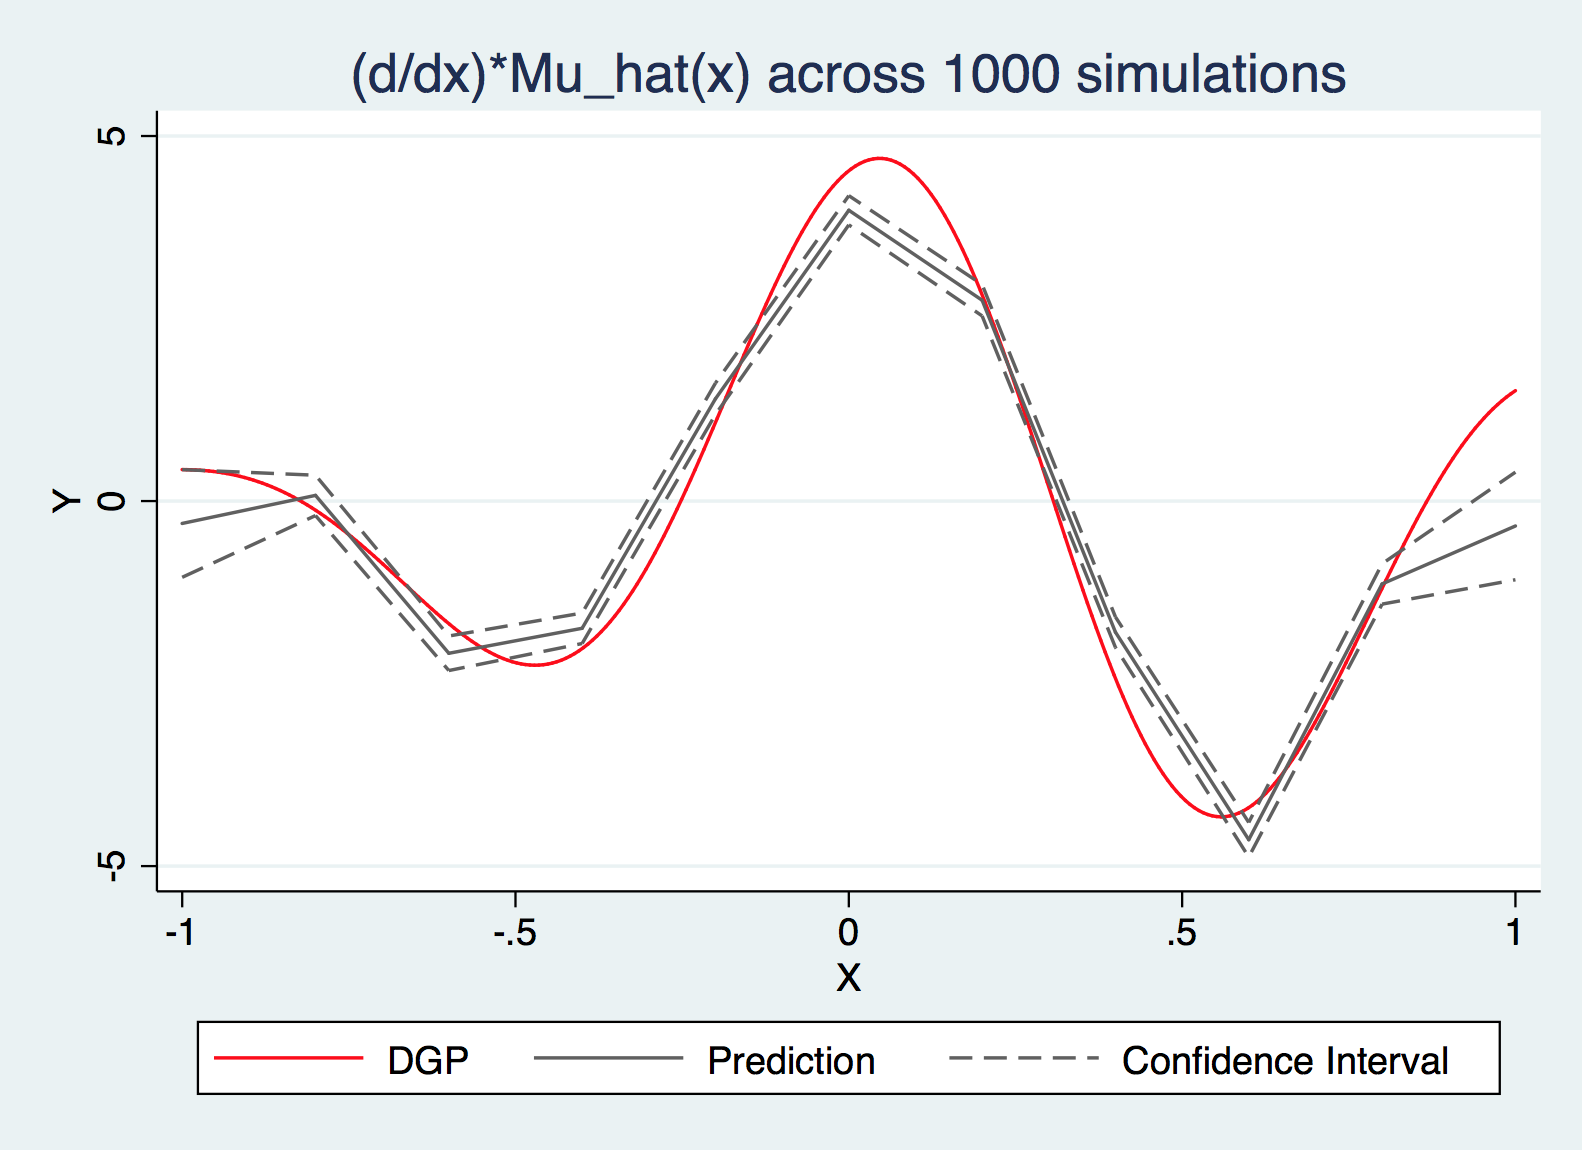
\includegraphics[totalheight=4cm]{pset2q2d.png}
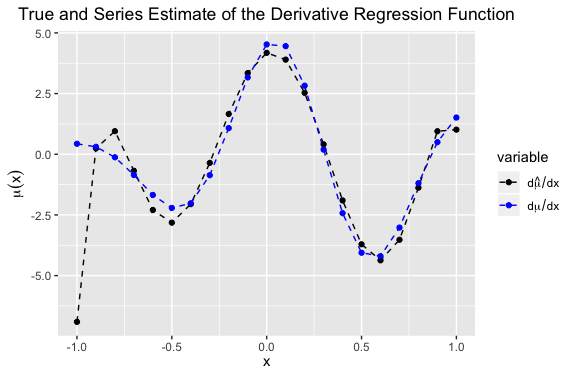
\includegraphics[totalheight=4cm]{pset2q2d_r.png}\\
The two kernel estimatation results from stata and R match up pretty closely. Although, the confidence interval was off for the stata code and I was unable to fix it before the deadline.
\newpage
\section{Semiparametric Semi-Linear Model}
\subsection{}

The following question concerns this moment condition:
\begin{gather*}
\E[(t_i - h_0(x_i))(y_i - t_i\theta)] = 0 \text{  , where }  h_0(x_i) = \E[t_i | x_i]
\end{gather*}

As long as $t_i$ is not collinear with $x_i$ then $\theta_0$ will be identifiable. Assuming that $\theta_0$ is identifiable, it satisfies the moment condition above:

\begin{gather*}
\E[t_i y_i] + \E[h_0(x_i)t_i\theta] - \E[h_0(x_i)y_i] - \E[t_i t_i\theta)] = 0 \\
\E[\E[t_i y_i |t_i, x_i]] + \E[\E[h_0(x_i)t_i\theta|t_i, x_i]]  - \E[\E[h_0(x_i)y_i |t_i, x_i]]  + \E[\E[t_it_i\theta) |t_i, x_i]]  = 0 \\
\E[h_0(x_i) \E[y_i |t_i, x_i]] + \E[h_0(x_i)h_0(x_i)]\theta  - \E[h_0(x_i) \E[y_i |t_i, x_i]]  + \E[h_0(x_i)h_0(x_i)]\theta   = 0 \\
0=0
\end{gather*}

To derive a closed form equation for $\theta_0$ we follow the steps outlined in Hansen's notes on nonparametrics (chapter 7), which describes Robinson (Econometrica, 1988).

\begin{gather*}
y_i = t_i\theta_0 + g(x_i) + \epsilon_i
\end{gather*}

First we take the conditional expectation with respect to the treatment and other covariates. (We assume the treatment is not collinear with the other covariates.)

\begin{gather*}
\E[y_i|t_i x_i] = \E[t_i|t_i x_i]\theta_0 + \E[g(x_i)|t_i x_i]  + 0
\E[y_i|t_i x_i] = h_o(x_i)\theta_0 + g(x_i) + 0
\end{gather*}

Next, let's define $ g_{y,x}  \coloneqq \E[y_i|t_i x_i]$, and subtract the equation above from the original regression.


\begin{gather*}
y_i - g_{y,x} = (t_i -  h_o(x_i))\theta_0 + g(x_i) - g(x_i) + \epsilon_i
\end{gather*}

Now, we can rewrite the regression as a residual regression:

\begin{gather*}
\epsilon_{yi} =  \epsilon_{ti}\theta_0 + \epsilon_i\\
y_i = g_{y,x} + \epsilon_{yi}\\
t_i =  h_o(x_i) + \epsilon_{ti}
\end{gather*}

Which produces the infeasible estimtor:

\begin{gather*}
\beta = \left( \sum\limits_{i=1}^n \epsilon_{ti} \epsilon_{ti}' \right)^{-1} \left( \sum\limits_{i=1}^n \epsilon_{ti} \epsilon_{yi}' \right)
\end{gather*}

Note that we can rewrite the residual regression as :

\begin{gather*}
M_{yx} y_i = M_{tx} t_i \theta_0 + \epsilon_i
\end{gather*}

Which is the second stage of an IV regression that partials out the effects of $X_i$ on $y_i$ and $t_i$ using anhilation matrixes.

\subsection{}
\subsubsection{}

If the treatment is undetermined by the power series of the covariates, $\theta_0$ is simply

\begin{gather*}
\theta_0 = (T'T)^{-1}(T'Y)
\end{gather*}

which has a feasible estimator of

\begin{gather*}
\hat{\theta}(K) =(\sum\limits_{i=1}^{n} t_i t_i)^{-1}  (\sum\limits_{i=1}^{n} t_i y_i)\\
\end{gather*}



\subsubsection{}
If the treatment is correlated to the other covariates, in order to estimate a feasible estimator, one must run Nadaraya - Watson kernel regressions of the outcome and treatment variables onto the power series.

\begin{gather*}
\hat{y}_i = \frac{\sum\limits_{i=1}^{n} k\left(\frac{p^{K_n}(x_i) - p^{K_n}(x)}{h}\right) y_i}{\sum\limits_{i=1}^{n} k\left(\frac{p^{K_n}(x_i) - p^{K_n}(x)}{h}\right)} \\
h_0(x_i) = \frac{\sum\limits_{i=1}^{n} k\left(\frac{p^{K_n}(x_i) - p^{K_n}(x)}{h}\right) t_i}{\sum\limits_{i=1}^{n} k\left(\frac{p^{K_n}(x_i) - p^{K_n}(x)}{h}\right)}
\end{gather*}

Now, construct residualize
\begin{gather*}
\hat{\epsilon}_{yi} = y_i - \hat{y}_i = M_{yx}y_i \\
\hat{\epsilon}_{ti} = t_i - h_0(x_i)   = M_{tx}t_i
\end{gather*}

Which produces the feasible estimator

\begin{gather*}
\hat{\theta}(K) = \left( \sum\limits_{i=1}^n \hat{\epsilon}_{ti} \hat{\epsilon}_{ti}' \right)^{-1} \left( \sum\limits_{i=1}^n \hat{\epsilon}_{ti} \hat{\epsilon}_{yi}' \right)
\end{gather*}


\subsection{}
\subsubsection{}
Fixing K, the reason this approach is called a "flexible parametric" estimation because you are estimating $\theta_0$, while letting

If $K\rightarrow\infty$ does not invalidate the "fixed K" assumption as long as the ratio between the observations and covariates is fixed $\left( \frac{K_n}{n} = \frac{\bar{K}}{\bar{n}}   \right)$

\subsubsection{}
Using the results above the confidence interval is

\begin{gather*}
CI_{95} = \left[\hat{\theta}(K)  - 1.96  \sqrt{\hat{V}_{HCO} / n}  ; \hat{\theta}(K) + 1.96  \sqrt{\hat{V}_{HCO} / n} \right]
\end{gather*}

\subsection{}


\end{document}
